\documentclass[12pt,english]{article}
\usepackage{mathptmx}
\usepackage{subcaption}
\usepackage{color}
\usepackage[dvipsnames]{xcolor}
\definecolor{darkblue}{RGB}{0.,0.,139.}
\usepackage[top=1in, bottom=1in, left=1in, right=1in]{geometry}
\usepackage{amsmath}
\usepackage{amstext}
\usepackage{amssymb}
\usepackage{setspace}
\usepackage{lipsum}
\usepackage[authoryear]{natbib}
\usepackage{url}
\usepackage{booktabs}
\usepackage[flushleft]{threeparttable}
\usepackage{graphicx}
\usepackage[english]{babel}
\usepackage{pdflscape}
\usepackage[unicode=true,pdfusetitle,
 bookmarks=true,bookmarksnumbered=false,bookmarksopen=false,
 breaklinks=true,pdfborder={0 0 0},backref=false,
 colorlinks,citecolor=black,filecolor=black,
 linkcolor=black,urlcolor=black]
 {hyperref}
\usepackage[all]{hypcap} 
\usepackage{breakurl}    



\linespread{2}

\begin{document}

\begin{singlespace}
\title{Geography's Impact on the Competitive Balance of the NBA}

\end{singlespace}

\author{Matt Mullins\thanks{ University of Oklahoma.\
E-mail~address:~\href{mailto:student.matthew.p.mullins-1@ou.edu}{matthew.p.mullins-1@ou.edu}}}


\date{April 26, 2018}

\maketitle

\begin{abstract}
\begin{singlespace}
This paper examines the impact of geographical location on each NBA team's chance of winning an NBA championship. I find no clear evidence to suggest that any single geographic variable tested in this paper significantly alters a teams championship prospect. However, I do find evidence that suggests that teams who are willing to spend more and pay the luxury tax improve their odds of winning significantly. These results suggest that teams who are aggressive in their spending fare better during the season, regardless of location.  
\end{singlespace}

\end{abstract}
\vfill{}

\pagebreak{}

\section{Introduction}\label{sec:intro}
For the past decade, a team led by Lebron James has won the Eastern Conference title. For the past 4 years, Las Vegas has made both the Cleveland Cavaliers and Golden State the favorites to make it to the championship game. As baseball and football begin to lose popularity, declining by by 10 and 2 percent respectively, the NBA has increased in popularity by nearly 3 percent and causing some sports experts to believe it will surpass the NFL as America's favorite sport \cite{abdul}. 
Because of its lower impact on athletes bodies and the fast pace that the game is played, the NBA has a very enticing product to offer fans. However, one key aspect they may be failing to address is the level of competition throughout the league. The NBA is currently being challenged by a strong competitive imbalance greater than any other US sports league. This imbalance can largely be attributed to the fact that the NBA is more star-driven than any other sports league, where an individual player can largely dictate the outcome of a game \cite{abdul}. The NBA has tried to establish a more level playing field using measures such a soft salary cap, where the cap is not absolute, allowing teams to exceed the limit and pay a luxury tax \cite{gomez}. In recent collective bargaining agreements the league has also introduced provisions that establish maximum salaries that give the drafting or home team a slight monetary advantage, but many of these provisions are tied to annual awards.
In theory, this equal distribution of revenue should have a positive impact on competitive balance, because it is addresses revenue disparity for smaller market teams and impacts a major variable that influences talent distribution. However, this assumption seems to be taken for granted with evidence pointing to the contrary. 
\newline
The NBA may be approaching a point where they will need to reconsider the equal spending structure of the league, and discover, as this research paper will attempt to do, if all else held relatively equal, teams in more desirable locations have been given an unfair advantage by the current rule book?
This analysis will be part of a growing number of economic papers attempting to better understand what impacts the competitive balance in sports. The primary variables that have been analyzed in previous research papers are players salaries and salary cap structures. This paper will take a different approach and instead an more urban economic analysis and try to attribute team success to the location where the club has been established. 
\newline
The primary statistical method that will be used to test this assumption will be a Bayesian approach. This method will allow us to use a powerful Hastings algorithm in conjunction with a Monte Carlo Markov Chain so that we can update our model constantly as it runs through 3 chains of simulations with data we will provide. Additionally, a classical OLS model will be used to test the same data and ensure that our estimators are tuned correctly in our Bayesian model. 
This papers primary contributions will be beneficial for all parties involved in the sport. For the league, understanding where they are deficient in terms of competitive balance will allow them to address the issue properly. For players, especially those who are considered middle and lower tier, this report will perhaps uncover whether they are being unfairly compensated by the league because of current cap limitations and lack of mobility. Finally, for the fans, this research should provide them to make an informed decision about whether or not they will want to continue supporting a local or favorite team, when other alternatives are available. 
\newline
This paper proceeds as follows. In the next section I will discuss passed works that have similarly touched on this issue or issues that are related in order to acknowledge their results, gain a better understanding of the labor environment and take away key ideas that may be beneficial for this current experiment. Following that, I will outline the relevant variables chosen for this research and the sources that they are collected from. After that, we will discuss the statistical methods used in further detail. Following that, we will provide our results from this research. Finally, we will state our actionable conclusions and point out any key lessons that should be taken away from this study. 




\section{Empirical Literature} \label{sec:litreview}
 
 Prior studies by \cite{davies}, \cite{owens}, \cite{helmut}, \cite{zimmer} and \cite{vrooman} have all taken different approaches to examining the competitive balance of professional sports and looked at how salary caps can impact that balance. 
 \newline
 Chris Davies, a lecturer from James Cook University's School of Law, discusses the implementation of salary caps in professional rugby, as well as analyzing the legality of salary caps in general. Davies is interested in understanding who salary caps or benefiting the most, whether they are legal in regards to the restraint of trade doctrine and whether salary caps are improving competition in these leagues. What Davies finds is that although the owners of the clubs benefit more by capping their total spending on salaries and players still benefit long-term because of greater stability in employment. He also concludes that in these leagues, the salary caps do seem to create and maintain healthy levels of competition, but it is worth noting that the money is allocated based on regions and other cost of living factors in these leagues \cite{davies}. 
 \newline
 Evan Totty and Mark Owens, in their 2011 paper on "Salary Caps and Competitive Balance in Professional Sports Leagues", use a similar statistical approach to examining competitive balance by performing linear panel regressions. However, their main variables of interest pertain to spending and salary caps. In their research they observe the NFL, NBA and NHL in order to get a more broad understanding of how these spending structures impact different leagues. What they find is that for these three leagues, salary caps have not improved competitive balance, and in fact, by looking at the standard deviations of winning percentages as a measure of competitive balance, find evidence that salary caps significantly decrease competitive balance across all of the leagues they observed \cite{owens}. 
 \newline
 Helmut Dietl, Markus Lang and Alexander Rathke find in their journal article titled: "The Effect of Salary Caps in Professional Team Sports on Social Welfare", that salary caps can increase or decrease social welfare depending on how competitive balance and aggregate talent is evaluated. For instance, if the league is already balance well in terms of competition levels (according to fans), then the introduction of a salary cap appears to reduce this level of balance. Alternatively, if the league examined suffers from an unequal distribution of its talent then a salary cap can help increase the social welfare pertaining to that league. Therefore, they conclude that salary caps are not as collusive as they appear on the surface and can be a useful mechanism in increasing the welfare of professional sports leagues \cite{helmut}. 
 \newline
 Timothy Zimmer, writing in the Sports Management International Journal, empirically tests how different levels of salary concentrations of teams in the NFL relate to success and what this means in regards to the leagues salary cap constrictions. After observing the 2000 - 2009 seasons in the NFL and using a fixed effect regression model to handle the unbalance panel data set he uses, Zimmer finds that teams must spend their total allotment of funds each season in order to maximize success each season. Also, the influence of salary cap concentration in the NFL appears to be non-linear in that either extremely high or extremely low salary concentrations provide the best probability of success. He finally notes that, in regards to the NFL, it is better to have fewer elite players than many good players \cite{zimmer}. 
 \newline
 Lastly, John Vrooman in his research titled: "The Economics of American Sports Leagues", examines the effects of labour constraints in professional sports and also seeks to discover whether the assumption that owners of sports clubs are profit maximizers holds. Interestingly, he finds that the payroll cap is a unique form of cost-sharing collusion and that its introduction into the NBA has created a sort of cartel of teams that act as a single firm. What this means is that the teams in the NBA appear to be most interested in profit maximizing for the league as a whole. This leads Vrooman to conclude that the NBA is least competitively balance league of the three major US professional sports \cite{vrooman}. 
 
 
 
 
 
\section{Data}\label{sec:data}
The primary two data sources for this research are ESPN and Statista. \newline
These two sources were chosen because of their reputation for accuracy and the abundance of data they collect and make available publicly. At times we will turn to other sources for when we are collection data and will make special note of this. The primary variable, which will be the dependent variable of this study will be Net Rating. Net Rating is a statistic that measures a team's point differential per 100 possessions (offensive rating - defensive rating). This variable is the primary focus because it gives an overall picture of how each team is performing both offensively and defensively. As would be expected, a team with a higher net rating has a greater chance of making the post season as shown in Figure 1 in the Plots and Charts section. The independent variables we will use to test our hypothesis include city size, denoted bigCity in our models. This variable measures the metropolis population for each team's home city and this is turned into a categorical variable using the mode of the data set. This data is collected from world population review's official website. Spending is denoted simply as spending in our models and is included to both confirm prior studies and further examine its role on a team's success. The third independent variable chosen is income tax, this one is chosen in order to determine if teams in locations with less income tax have a distinct advantage over teams with higher income tax rates, given the equal limits on spending teams are faced with under the soft cap. It is depicted as incomeTax in our models. This data is collected from the tax foundations website. Next, we will use the average annual temperature of each state as a variable, denoted as avgTemp, in order to test whether teams with more moderate climates more easily attract top talent and thus have a higher net rating. Weather data is gathered from the National Climate Data organization. The fifth dependent variable used in our research is management ranking, manageRank. There is a chance that coaches and owners are attracted to desirable locations and would in-turn receive a higher ranking from ESPN. Therefore, we are testing to see if there is correlation with this variable and others in our model, and also to see if management and coaching ranks have an impact on how well the team performs. We will further explore team spending on performance and will categorically differentiate teams based on whether or not they pay luxury tax. This categorical variable is denoted luxuryTax. Since we are researching the geographical impact on team success, we will test to see if teams who travel more in a season are at a disadvantage. This variable would seem to favor more central teams, putting teams on the coast at a disadvantage in total miles traveled, depending on schedule. It will be tested using the variable - miles. Also, there is a chance certain cities have more passionate or supportive fans than others, and we will attempt to test whether or not teams who are given more fan support respond with better performances on the court. The best way we can test this is by testing the total number of fans that a team receives at home over the course of a year, denoted fanAttend. The second to last variable we examine is ticket price, which is a good indicator of both the teams popularity, usually correlated with higher prices, and the affluence of the area that the team is located. By testing this variable, we will see if teams who are charging more per ticket are producing the results we would expect on the court. This variable is denoted as ticketPrice. Finally, the last variable we are interested in examining is each cities crime. The hypothesis of this is that players, coaches and owners with more mobility options will settle in places with less crime. We will test to see if this is true and whether or not it translates to success on the basketball court. This data is gather from City-Data.
There are many other variables that could also be included such as housing prices, investment opportunities and an athletes home-town. These and other variables that impact Net-Rating are theoretically captured by the error term epsilon in this study. 




\section{Empirical Methods}\label{sec:methods}
The two primary methods that this report will use to conduct experiments will be the frequentest approach, a general linear model, as well as Bayesian inference methods. 
The Ordinary Least Squared Model can be depicted in the following equation:
\begin{align*}
    \label{eq:1}
netRTG_{i} \sim \alpha_0 + \ beta1 * bigCity_{i}\ + \ beta2 * spending_{i} \ + \ beta3 * incomeTax_{i} \\
+ \ beta4 * avgTemp_{i} \ + \ beta5 * manageRank_{i} \ + \ beta6 * luxuryTax_{i} \ + \ beta7 * miles_{i} \\ + \ beta8 * fanAttend_{i}\ + \ beta9 * ticketPrice_{i} \ +  \ beta10 * crimeIndex_{i} + \epsilon_{i}
\end{align*}
The Bayesian analysis will consist of using a Gibbs Sampling approach. Gibbs sampling is a special case of the Metropolis-Hastings algorithm, which is an algorithm that allows the user to create a posterior distribution in complex models where it is difficult to explicitly solve the integral in Bayes' rule. Using this technique, we will obtain samples from the posterior distribution by first cycling through each of the parameters in a sequenced  order. We do this instead of a random walk approach because it would take too many steps to visit every variable in our model by random selection. Once the parameter is selected, Gibbs sampling then assigns a value for the parameter by generating a random value chosen directly from the conditional probability distribution. Combined with the other unchanged values, this is now the new position in the random walk. Now that we have generated a random value for our first parameter, we conditionalize on it and now determine the conditional distribution for our next parameter. We then conditionalize on the new value of this parameter and the cycle continues. The sampling of each parameter with all others held constant is shown mathematically:
\begin{align*}
\label{eq:2}
Initialize: x^{(0)} \sim q(x)\\
for: i = 1, 2, ...do\\
x_1^{(i)} \sim p(X_1 = x_1| X_2 = x_2^{(i-1)}, X_3 = x_3 ^{(i-1)},...,X_D = x_D^{(i-1)})\\
x_2^{(i)} \sim p(X_2 = x_2| X_1 = x_1^{(i-1)}, X_3 = x_3 ^{(i-1)},...,X_D = x_D^{(i-1)})\\
x_D^{(i)} \sim p(X_D = x_D| X_1 = x_1^{(i-1)}, X_2 = x_2 ^{(i-1)},...,X_D = x_D^{(i-1)})
\end{align*}
The posterior distribution will now be a product of the conditional posterior distributions for each parameter. Mathematically, because the posterior is the product of these independent beta and binomial distributions we can show:
\begin{align*}
    \label{eq:3}
   p(\theta_1|\theta_2,D) = p(\theta_1,\theta_2|D)/p(\theta_2|D)\\
    = p(\theta_1,\theta_2|D) / \int d\theta_1 p(\theta_1,\theta_2|D)\\
p(\theta_1|\theta_2,D) = p(\theta_1,\theta_2|D)/\int d\theta_1p(\theta_1,\theta_2|D)\\
= \frac{beta(\theta_1|z_1+a_1, N_1-z_1+b_1)beta(\theta_2|z_2+a_2,N_2-z_2+b_2)}
{\int d\theta_1 beta(\theta_1|z_1+a_1, N_1-z_1+b_1)beta(\theta_2|z_2+a_2,N_2-z_2+b_2)} \\
= \frac{beta(\theta_1|z_1+a_1, N_1-z_1+b_1)beta(\theta_2|z_2+a_2,N_2-z_2+b_2)}{beta(\theta_2|z_2+a_2, N_2-z_2+b_2) \int d\theta_1beta(\theta_1|z_1+a_1,N_1-z_1+b_1)} \\
= \frac{beta(\theta_1|z_1+a_1, N_1-z_1+b_1)beta(\theta_2|z_2+a_2,N_2-z_2+b_2)}{beta(\theta_2|z_2+a_2, N_2 - z_2 + b_2)} \\
beta(\theta_1|z_1+a_1, N_1 - z_1 +b_1)
\end{align*}
In the long run our Gibbs sampler will converge to the same distribution as the Metropolis algorithm. But we will use Gibbs sampling in our case because of greater efficiency. One disadvantage to note. Because we are only changing one parameter value at a time we run the risk of encountering various correlation concerns. 
The model that will be used for Our Gibbs Sampling Approach will be:
\begin{align*}
\label{eq:4}
netRTG[i] \sim dnorm(\mu[i], \tau)\\
Where: \mu[i] \sim beta0\ + \ beta1 * bigCity_{i}\ + \ beta2 * teamSpending_{i} \ + \ beta3 * incomeTax_{i} \\ + \ beta4 * avgTemp_{i} \ + \ beta5 * manageRank_{i}\ + \ beta6 * luxuryTax_{i} \ + \ beta7 * miles_{i} \\ + \ beta8 * fanAttend_{i}\ + \ beta9 * ticketPrice_{i} \ +  \ beta10 * crimeIndex_{i}
\end{align*}
Where Tau is the precision term:
\begin{align*}
\label{eq:5}
\tau = \frac{1}{\mu^{2}}
\end{align*}
For this model we will assume apriori independence and will assign low impact, stochastic priors as to avoid any subtle bias:
\begin{align*}
\label{eq:6}
    beta0 \sim dnorm(0.0, 1.0^{-6})\\
	beta[i] \sim dnorm(0.0, 1.0^{-6})\\
	sigma \sim dunif(0, 1000)
\end{align*}
Finally, by using this Gibbs Sampling approach as discussed above, we will be able to construct our posterior distribution using the joint probabilities found from sampling using and MCMC technique. This enables us to properly implement Bayes Theorem, shown below:
\begin{align*}
\label{eq:7}
    Bayes: p(\theta|x) = \frac{p(\theta)p(x|\theta)}{p(x)} 
\end{align*}



\section{Findings}\label{sec:findings}

The results from the OLS model are shown in Table 2 in the Charts and Data section of this report. Also, the Bayesian results can be found in Table 1 of the same section. 
\newline
We begin with the OLS regression to see which variables this model reports as most significant before discussing our Bayesian results. We find five variables that show different levels of meaningful significance: Management Rank, Spending, Luxury Tax, Fan Attendance and Crime Index. Management Rank, with a P value of less than 0.1 percent appears to be the most statistically significant variable in this classical model. With a coefficient of 1.889, it indicates that on the ESPN scale from 0-10, as a teams management ranking improves by 1 total point, it leads to an improvement of 1.889 to a teams Net Rating, which is significant. Luxury Tax is also shown to be a meaningful estimator with a P value less than 0.1 percent. With a beta hat value of 3.057, this indicates that for the teams that are willing to spend above the cap limits and pay the luxury tax, they are seeing a 3.057 Net Rating improvement compared to teams not paying luxury tax. Additionally, Spending has a P value of less than 1 percent in this regression. This result has been researched extensively and will not be examined much further in this report. It should also be mentioned that Crime Index and Fan Attendance both showed P values of less than 10 percent. 
\newline
Next we look at Table 1, the results from the Gibbs Sampler, our Bayesian method for finding point estimators. In order to better understand which variables are significant, we first turn to the Bayesian Credible Intervals (BCI) reported in Panel B of the table. For the intervals that include 0 within the BCI, we are able to rule them out as most likely not being statistically significant. The remaining variables not ruled out from this test are: spending, manageRank, luxuryTax. 
\newline
Next we look to the MCMC diagnosis for each of the independent variables shown in the charts found in the Plots and Charts section below. Beta 1, which is the variable for a large city, shows healthy iterations, low auto-correlation, its Gelman-Rubin statistic approaches 1 and its 3 MCMC chains show strong signs of convergence. However, despite these healthy diagnostics, we cannot qualify this variable as significant still. 
\newline
Beta6, representing luxury tax, also shows very healthy MCMC diagnostics, similar to Beta1 described above. It indicates, nearly identically to the OLS model, that teams paying luxury tax increase Net Rating by 3.054. We are comfortable labeling this variable as significant after seeing the test results from both models. 
Next, looking at Beta5 for management ranking, we see healthy iterations and convergence of the 3 chains, however, we see a high level of auto-correlation and this indicates we would need to do further testing with this variable before determining if it stands alone as significant. 
Finally, looking at the spending variable, beta2, we observe variance in both the iterations and the shrinkage factor, in addition to an indication of potential auto-correlation in our model. Because of this, it is uncertain whether we can say with a high probability that spending is significant. 



\section{Conclusion}\label{sec:conclusion}

This research seeks to discover whether geographical differences significantly impacts the competitive balance of the NBA. It has been shown by prior research that the salary cap structure of the NBA is causing a competitive imbalance in the league and my hypothesis is that geography further exacerbates this problem. To perform the analysis, I use two different statistical modeling techniques to test ten unique variables that relate to each NBA team from the past 6 regular seasons. After testing these variables using a classic OLS approach and a Bayesian Gibbs Sampler approach, I am able to obtain a relatively clear picture as to whether or not any of these hypothesized variables are in fact a significant factor in the competitive imbalance. In this report, I find no evidence that would clearly indicate that certain aspects of geography are significantly impacting the competitive balance of the league. Of the variables tested, Crime Index is the only geographical one that shows significance, from the results in the OLS model, but this is not supported by the Bayesian model and inconclusive as to its impact on net rating. Furthermore, variables including weather and city size seem to have null effects on a teams net rating in both the OLS and Bayesian model, which further disproves some of my urban economic theories that suggest human capital relocates to certain desirable locations when pay is nearly equal. 
\newline
Although my hypothesis is proven incorrect by this study, it importantly shows that geography and city size should be less of a concern for the NBA league when it considers relocating and expanding its teams. These results are also an important finding that will provide both the NBA league office and its club owners with invaluable data to use as they continue looking for ways to improve the level of competition. First, since variables such as weather and income tax do not have the impact that this study hypothesized, this indicates that players may be clustering in certain locations because of other factors not related to geography. This could include a teams recent momentum, the players hometown, etc.  
\newline
In order to improve upon this type of study in the future I would advise collecting a larger sample of data in which to run these statistical models. The cyclical nature of teams in the NBA means that it is likely some of the results can be attributed to the sample only capturing a single NBA cycle where some teams are up and some are down, and not truly capturing the longer-term trends that some of these variables would be more suited to predict. I would also like to expand this study to include other sports leagues to further increase the scope and data points that can be used to tune each of the chosen variables.
\newline
Finally, I think the largest beneficiary of this study is the fan. By providing evidence that suggests geography is not a major factor impacting the balance of the NBA, teams in small and large markets alike should feel comfortable knowing that the their local teams are not being disadvantaged because of their location and this means that teams do not need to be uprooted in order to increase their odds of winning.


%---------------------
% References
%_____________________

\pagebreak{}
\begin{spacing}{1.0}
\bibliographystyle{jpe}
\bibliography{NBA.bib}
\addcontentsline{toc}{section}{References}
\end{spacing}
\vfill
\pagebreak{}
\clearpage




%--------------------------
% Table Results
%--------------------------

\section{Plots and Charts}\label{sec:data}

\begin{table}[ht]
\caption{Bayesian Summary Statistics of Variables of Interest}
\label{tab:descriptives} 
\centering
\begin{tabular}{lccc}
&&&&\\
\multicolumn{5}{l}{\emph{Panel A: Summary Statistics for Variables of Interest}}\\
\toprule
            Variable & Mean  & Std. Dev. & Naive SE    \\
\midrule
 Intercept & -28.03 & 0.2425 & 0.01283 \\ 
 bigCity & -0.1156 & 0.007159 & 2.117E -03  \\ 
 spending & 5.164E-08 & 5.473E-10 & 7.382E -11\\
 incomeTax & -3.871 & 0.06025 & 0.01255 \\
 avgTemp & 0.05735 & 0.001184 & 1.233E -04 \\
 manageRank & 1.892 & 0.009734 & 0.00104 \\
 luxuryTax & 3.054 & 0.0103 & 0.00296 \\
 miles & 0.000054 & 0.000003 & 2.027E -07 \\
 fanAttend & 0.000007 & 1.738E-7 & 1.363E -08  \\
 ticketPrice & 0.002469 & 0.000077 & 2.165E -05 \\
 crimeIndex & 0.003873 & 0.000042 & 7.057E -06  \\
 sigma & 4.201 & 0.001134 & 7.347E -04
&&&&\\
\multicolumn{5}{l}{\emph{Panel B: Bayesian Credible Interval Results}}\\
\midrule
                            Variable & 2.5 Percent & 97.5 Percent  \\
\midrule
Intercept  & -36.23 & -20.31\\
bigCity  & -1.432 &  1.197\\
spending   & 4.609E -09  & 9.675E -08\\
incomeTax & -11.53 & 4.095\\
avgTemp & -0.0165 &  0.1366\\
manageRank & 1.274 & 2.573\\
luxuryTax &  1.210 & 4.900\\
miles & -6.950E -05  & 1.803E -04\\
fanAttend &  -1.070E -06 &  1.588E -05\\
ticketPrice  & -0.01099 & 0.01576\\
crimeIndex & -5.945E -04  & 8.170E -03\\
sigma  &  3.778   & 4.686 

\bottomrule
\end{tabular}

\footnotesize Note: If the 95 Percent BCI includes 0, this indicates the variable is insignificant
\end{table}


\begin{table}[ht]
\caption{OLS Summary Statistics of Variables of Interest}
\label{tab:descriptives} 
\centering
\begin{tabular}{lccc}
&&&&\\
\multicolumn{5}{l}{\emph{Panel A: OLS Summary Statistics}}\\
\toprule
  Variable & Mean  & Standard Error & P-Value   \\
\midrule
Intercept & -28.04 & 4.031 & 7.34E-11***   \\ 
 bigCity & -0.1152 & 0.6630 & 0.86230   \\ 
 spending & 5.17E+08 & 2.292E -08 & 0.02537*  \\
 incomeTax & -3.885 & 3.913 & 0.32219  \\
 avgTemp & 0.05753 & 0.03869 & 0.13888  \\
 manageRank & 1.889 & 0.3270 & 3.57E-08***  \\
 luxuryTax & 3.057 & 0.9256 &  0.00117**  \\
 miles & 0.000055 & 6.156E -06  &  0.37204 \\
 fanAttend & 0.000007 & 4.135E -03 & 0.07735 .  \\
 ticketPrice & 0.002495 & 6.714E -03 & 0.71063  \\
 crimeIndex & 0.003854 & 2.209E -03 & 0.08291 . 
&&&&\\
\bottomrule
\end{tabular}

\footnotesize Significance Levels: 0 ‘***’ 0.001 ‘**’ 0.01 ‘*’ 0.05 ‘.’ 
\end{table}




%------------------------
% Plots and Graphs
%------------------------

\begin{figure}[ht]
\caption{Relationship of NetRating with making the playoffs}
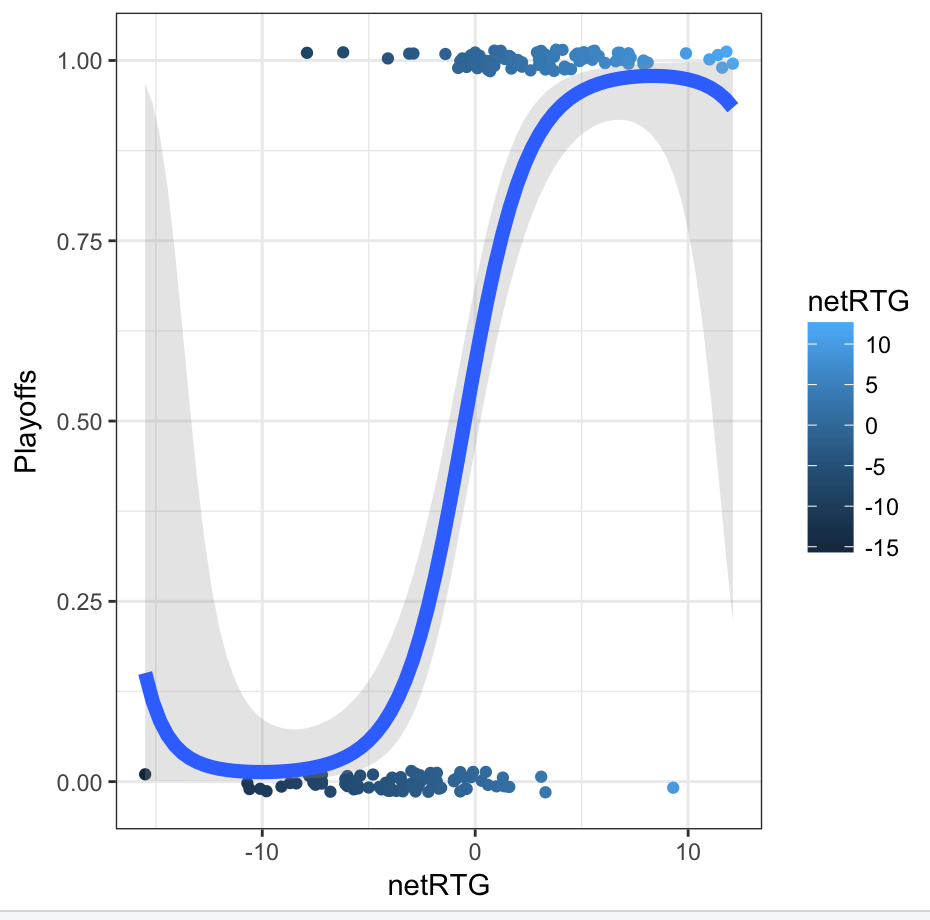
\includegraphics[scale=0.5]{Initial1.png}
\centering
\end{figure}

\begin{figure}[ht]
\caption{Regular seasons wins related to the teams annual average temperature }
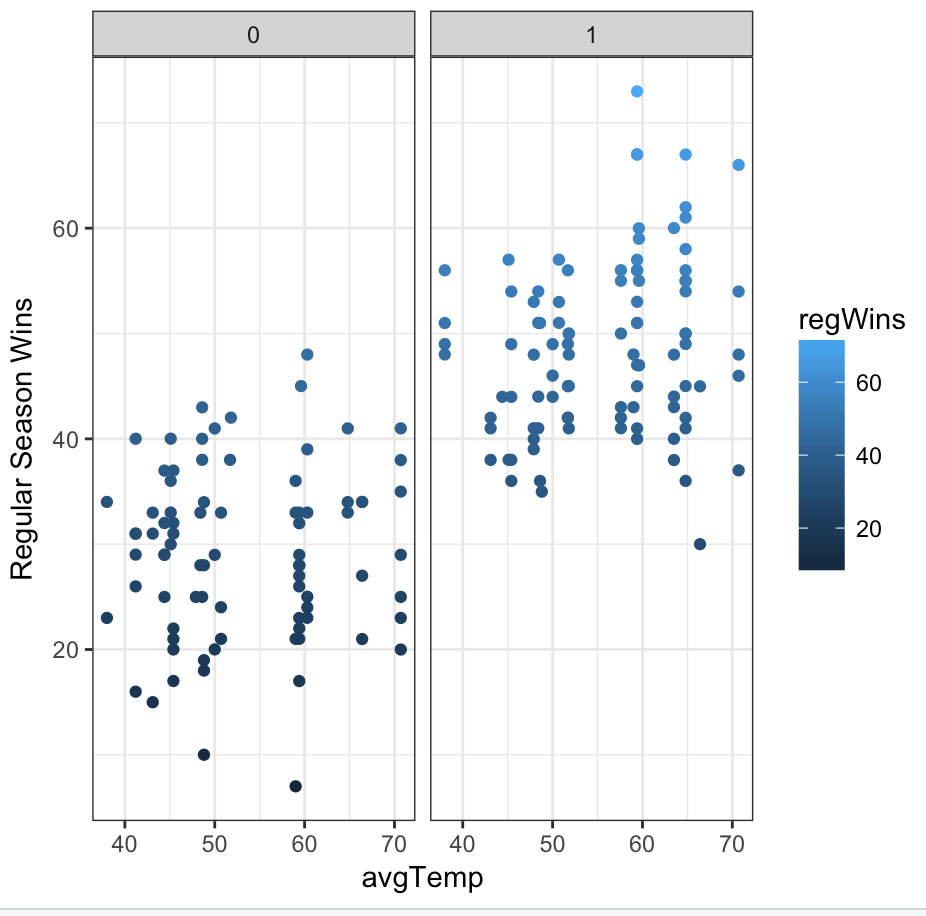
\includegraphics[scale=0.5]{Initial2.png}
\centering
\end{figure}

\begin{figure}[ht]
\caption{Luxury tax, net rating and the outcome of making playoffs }
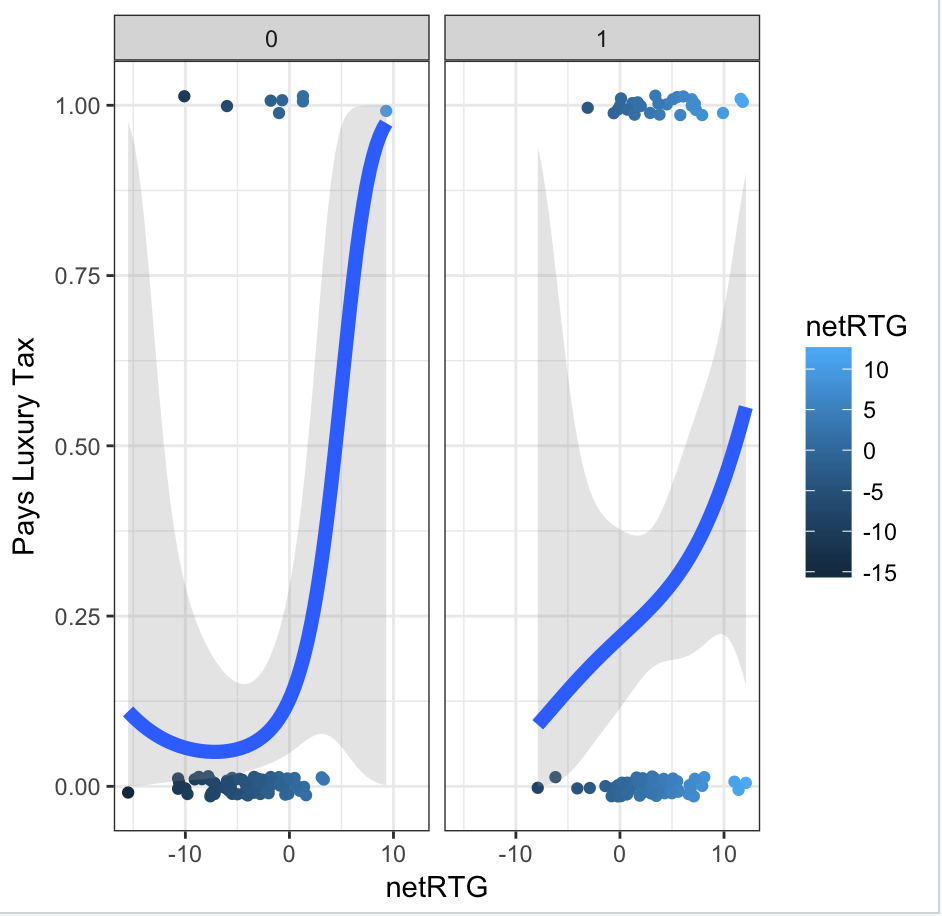
\includegraphics[scale=0.5]{Initial3.png}
\centering
\end{figure}

\begin{figure}[ht]
\caption{JAGS Model}
\includegraphics[scale=0.5]{Jags Model.png}
\centering
\end{figure}

\begin{figure}[h]
\caption{MCMC Chains 1-3 for each variable }
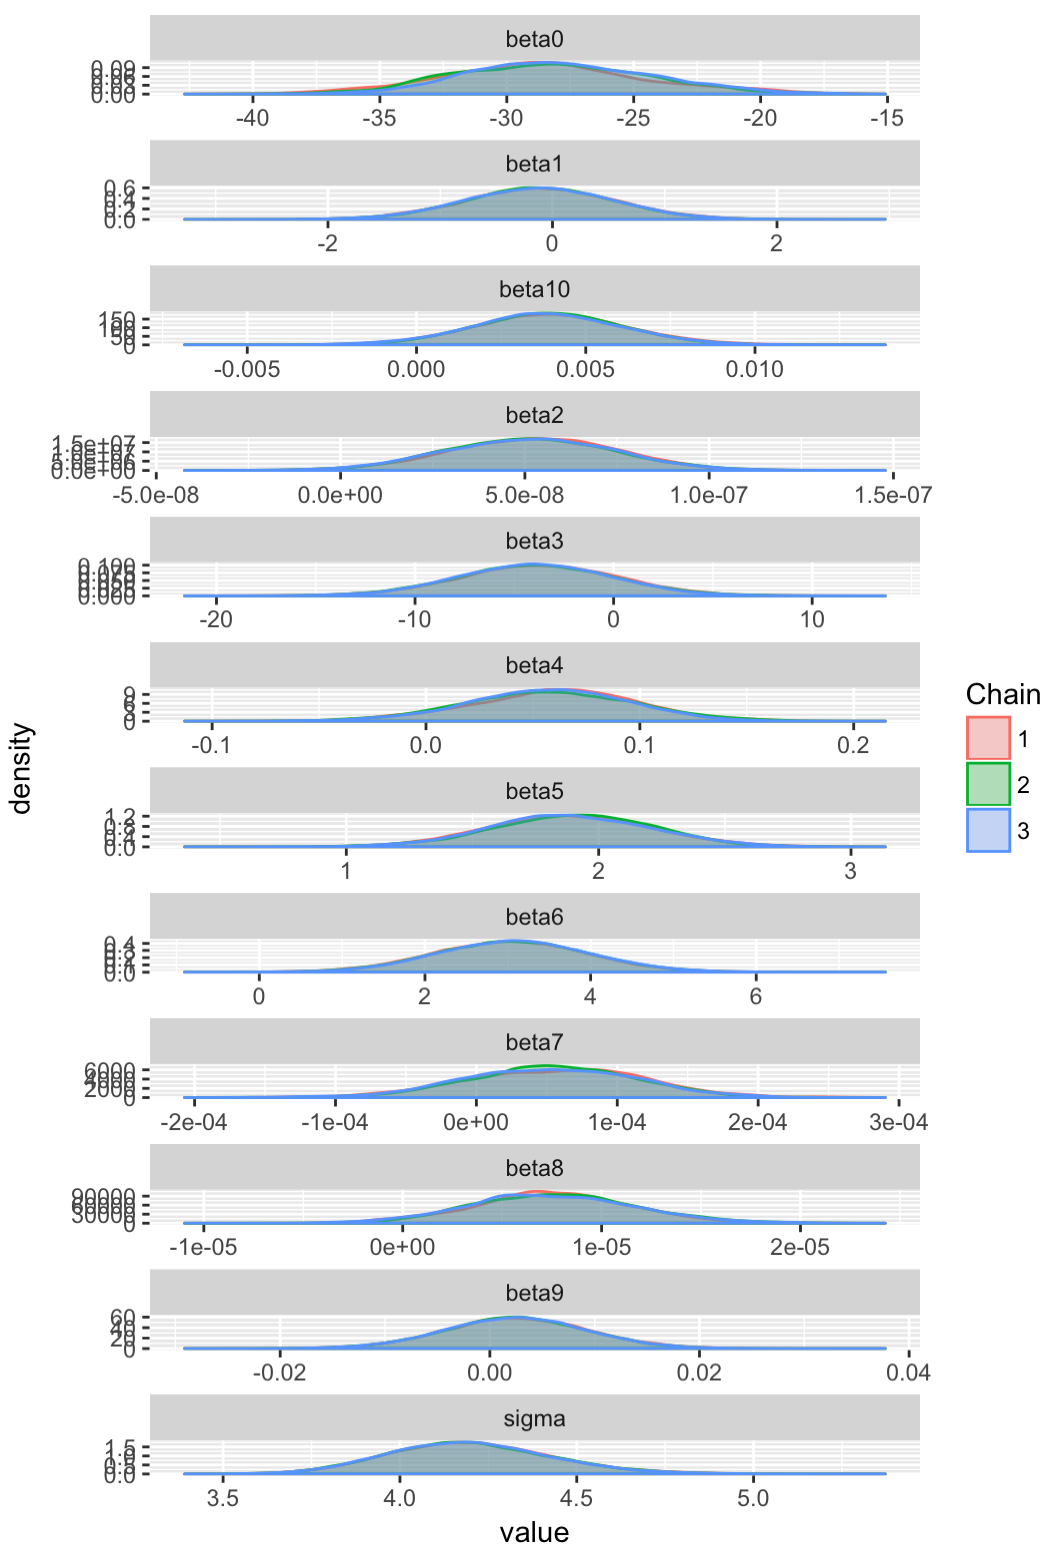
\includegraphics[scale=0.5]{Chains.png}
\centering
\end{figure}

\begin{figure}[h]
 
\begin{subfigure}{0.5\textwidth}
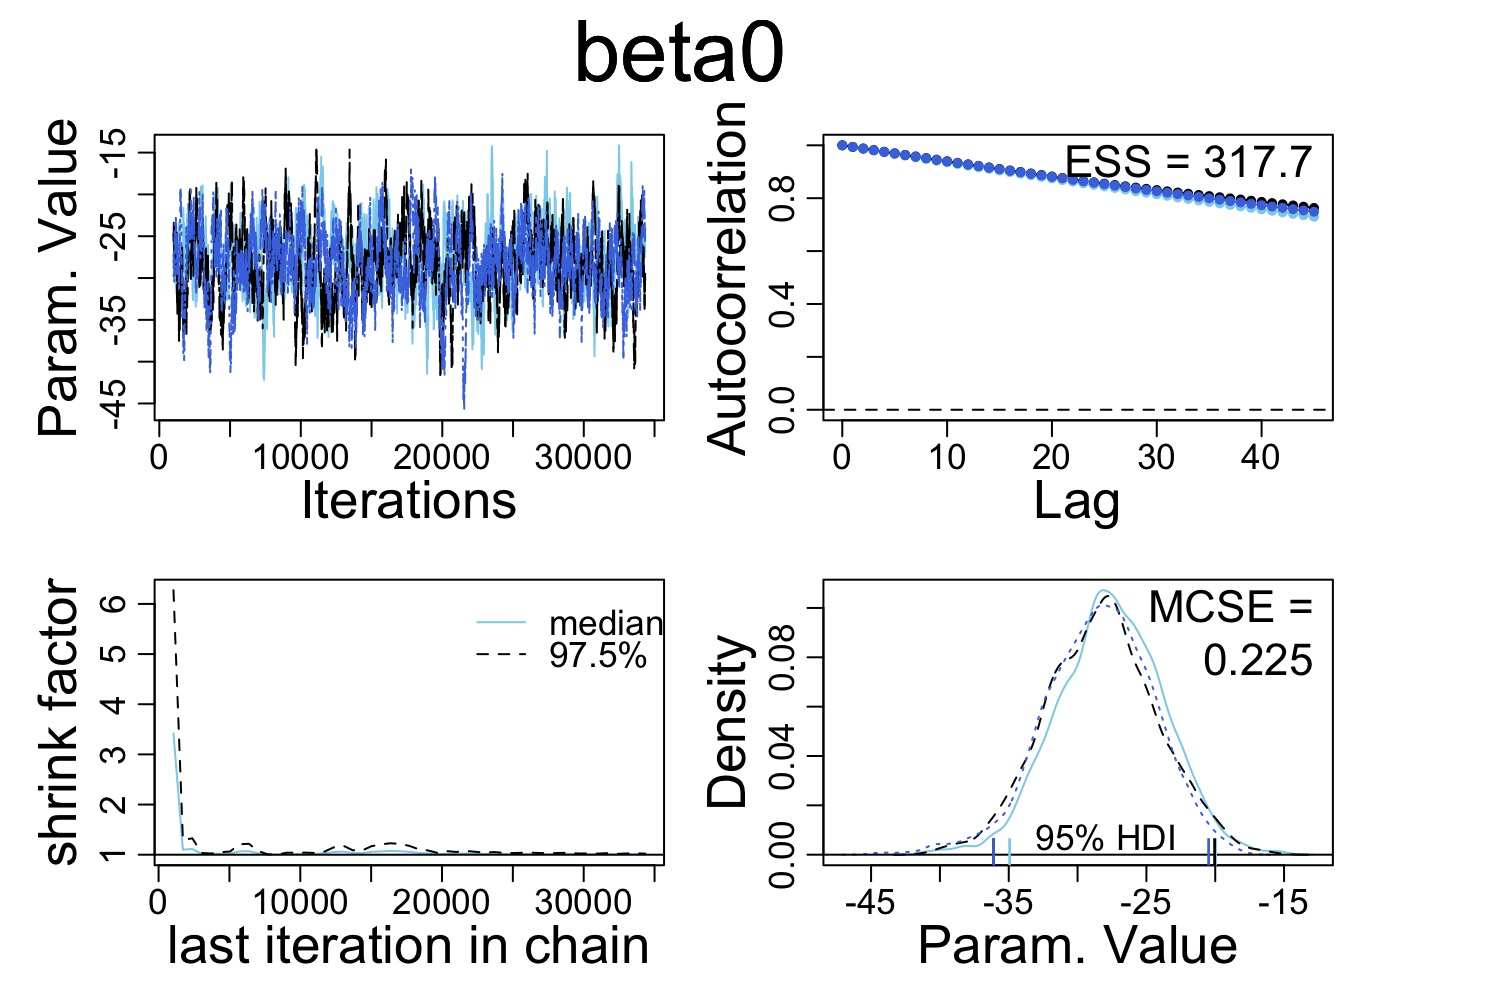
\includegraphics[scale = 0.25]{beta0.png} 
\caption{Intercept}
\label{fig:beta0}
\end{subfigure}
\begin{subfigure}{0.5\textwidth}
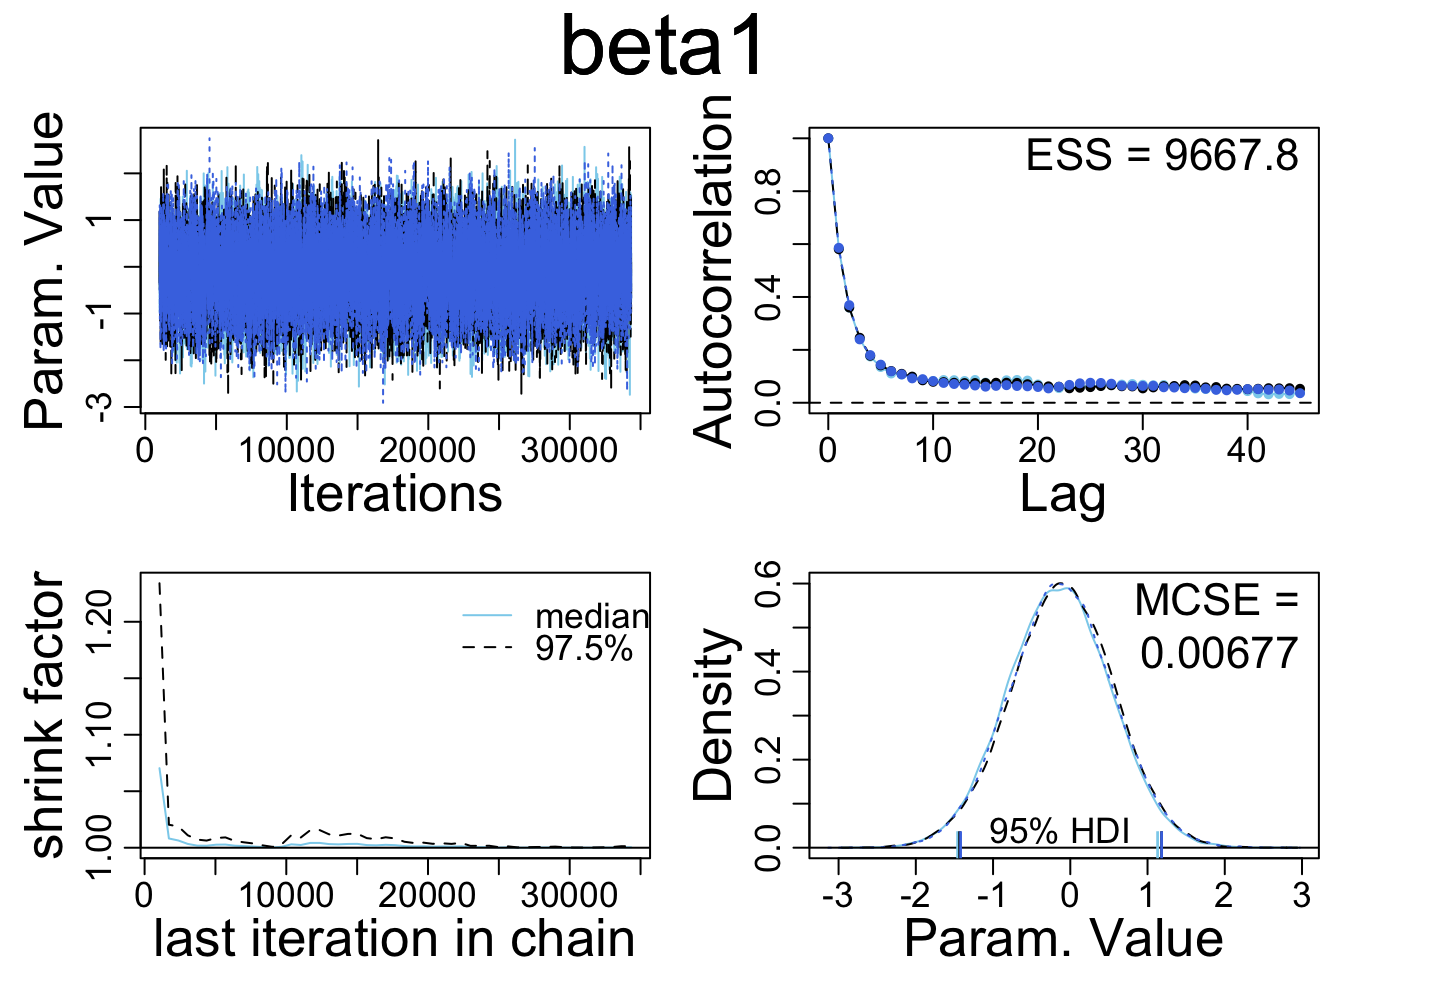
\includegraphics[scale = 0.25]{beta1.png}
\caption{Big City}
\label{fig:subim2}
\end{subfigure}
\label{fig:beta1}
\end{figure}

\begin{figure}[h]
 
\begin{subfigure}{0.5\textwidth}
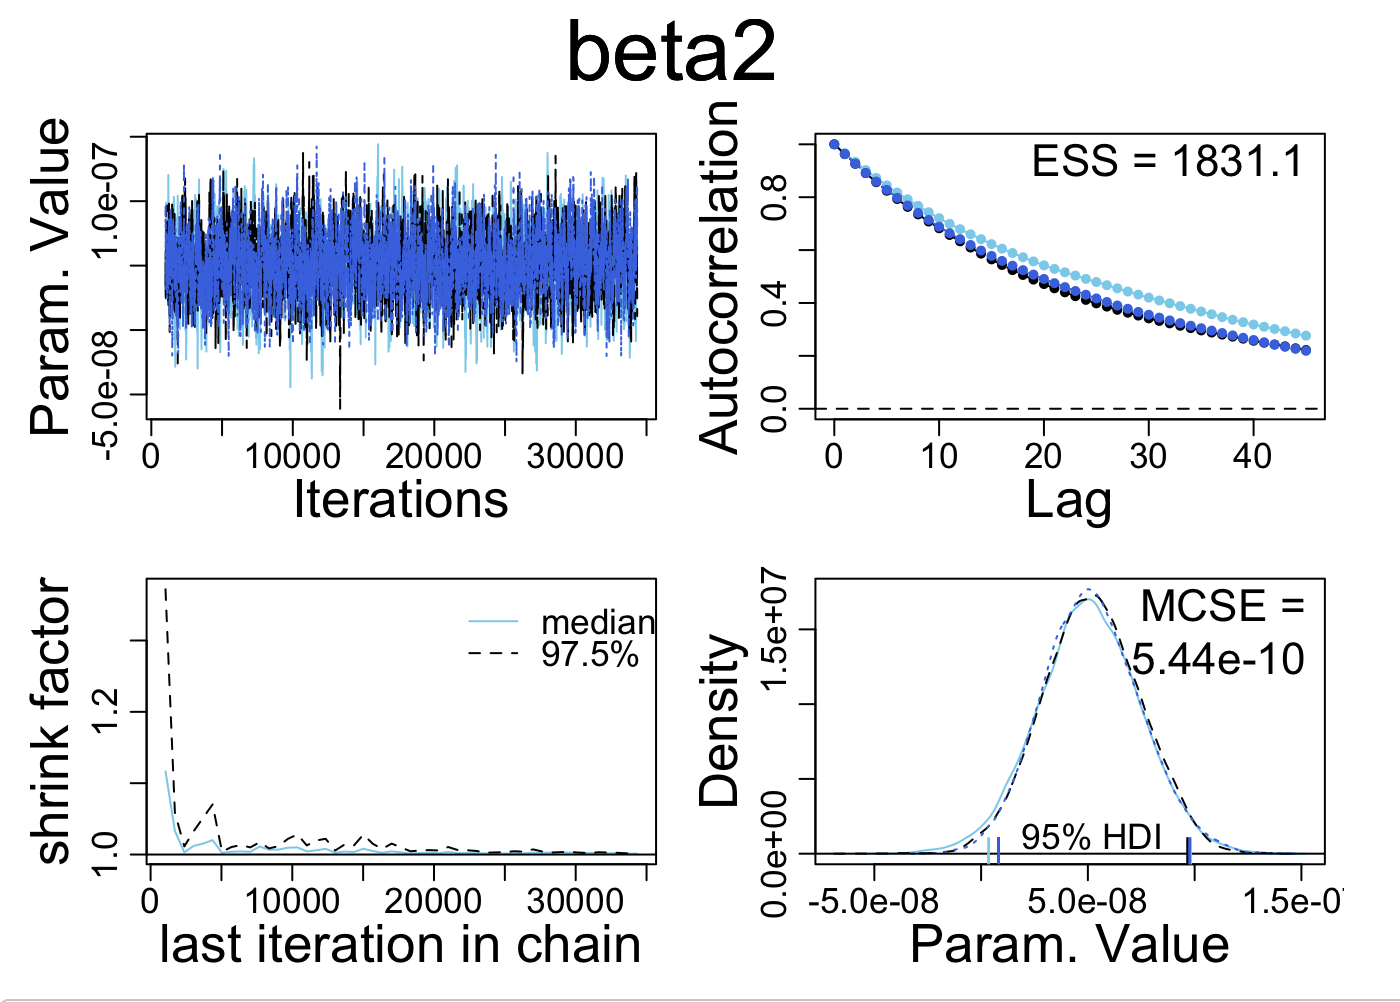
\includegraphics[scale = 0.25]{beta2.png} 
\caption{Spending}
\label{fig:beta2}
\end{subfigure}
\begin{subfigure}{0.5\textwidth}
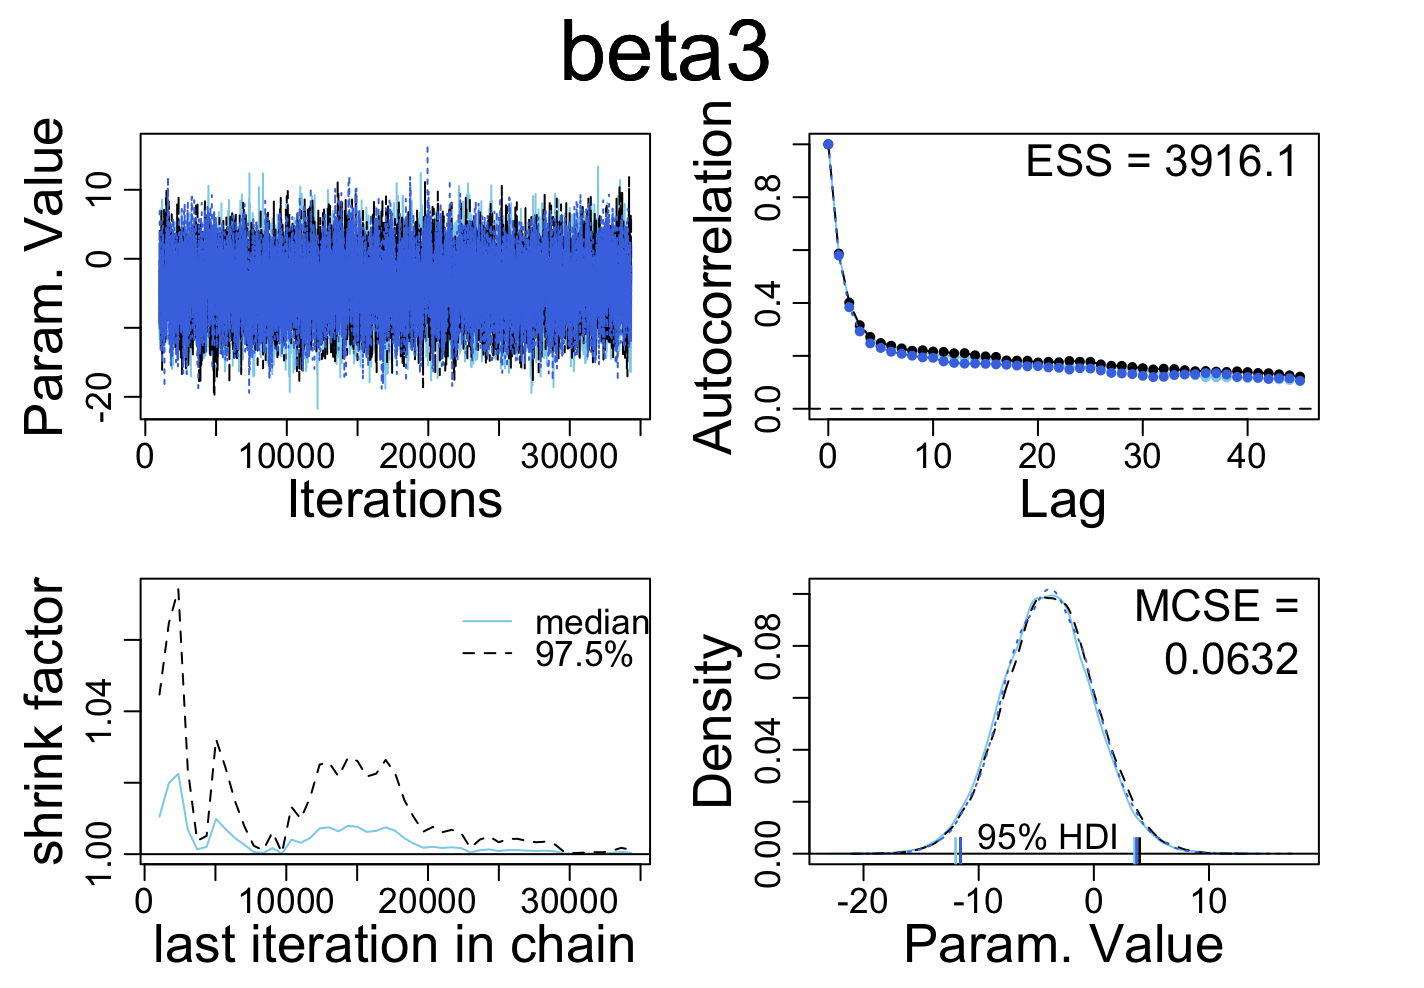
\includegraphics[scale = 0.25]{beta3.png}
\caption{Income Tax}
\label{fig:beta3}
\end{subfigure}
\label{fig:beta2}
\end{figure}

\begin{figure}[h]
 
\begin{subfigure}{0.5\textwidth}
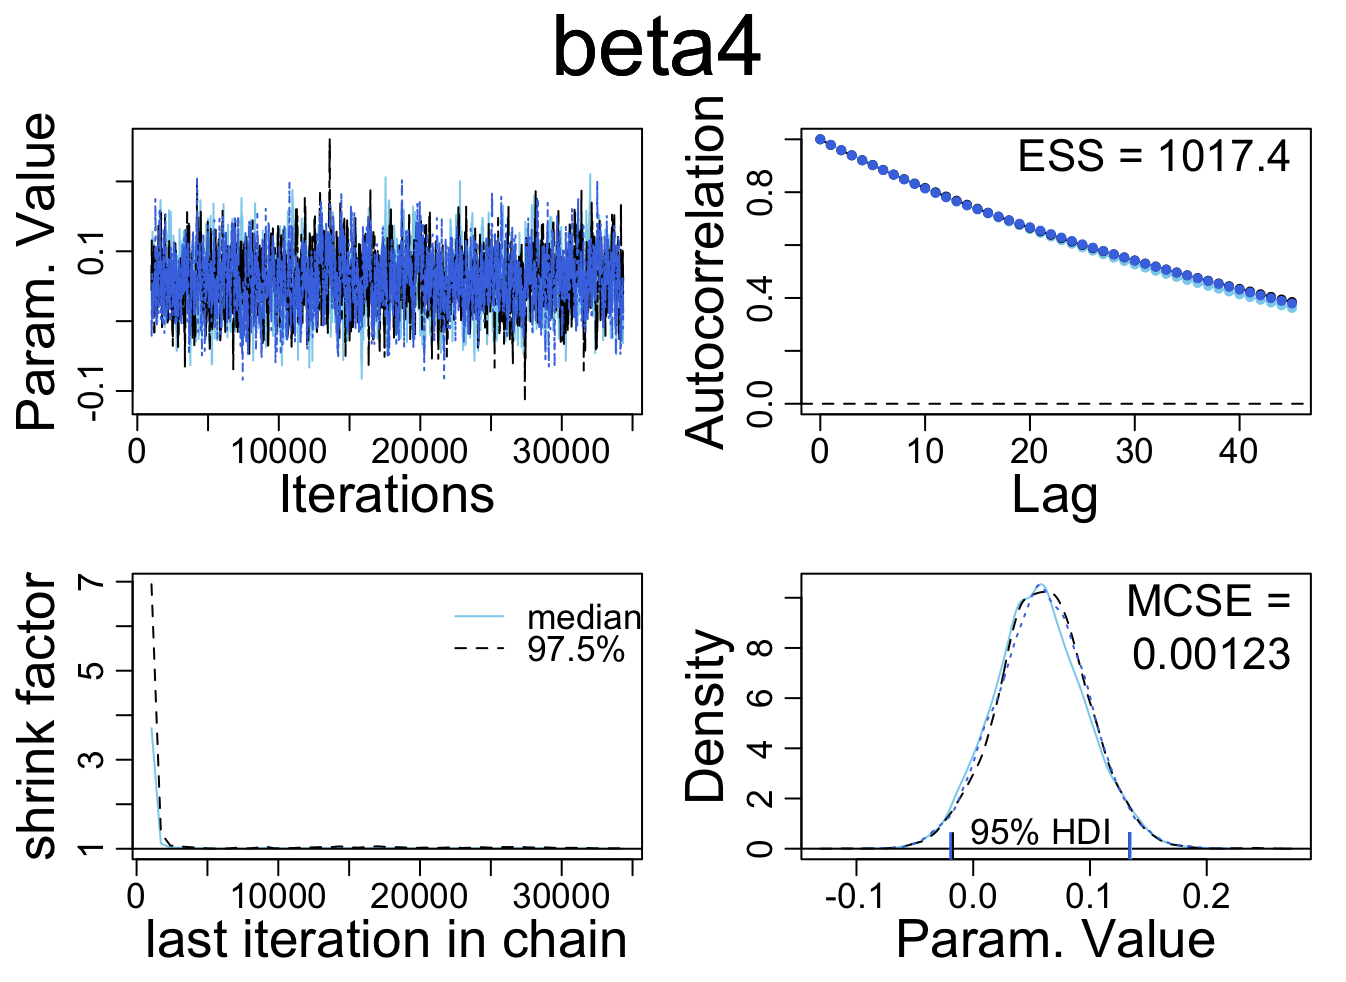
\includegraphics[scale = 0.25]{beta4.png} 
\caption{Average Temperature}
\label{fig:beta0}
\end{subfigure}
\begin{subfigure}{0.5\textwidth}
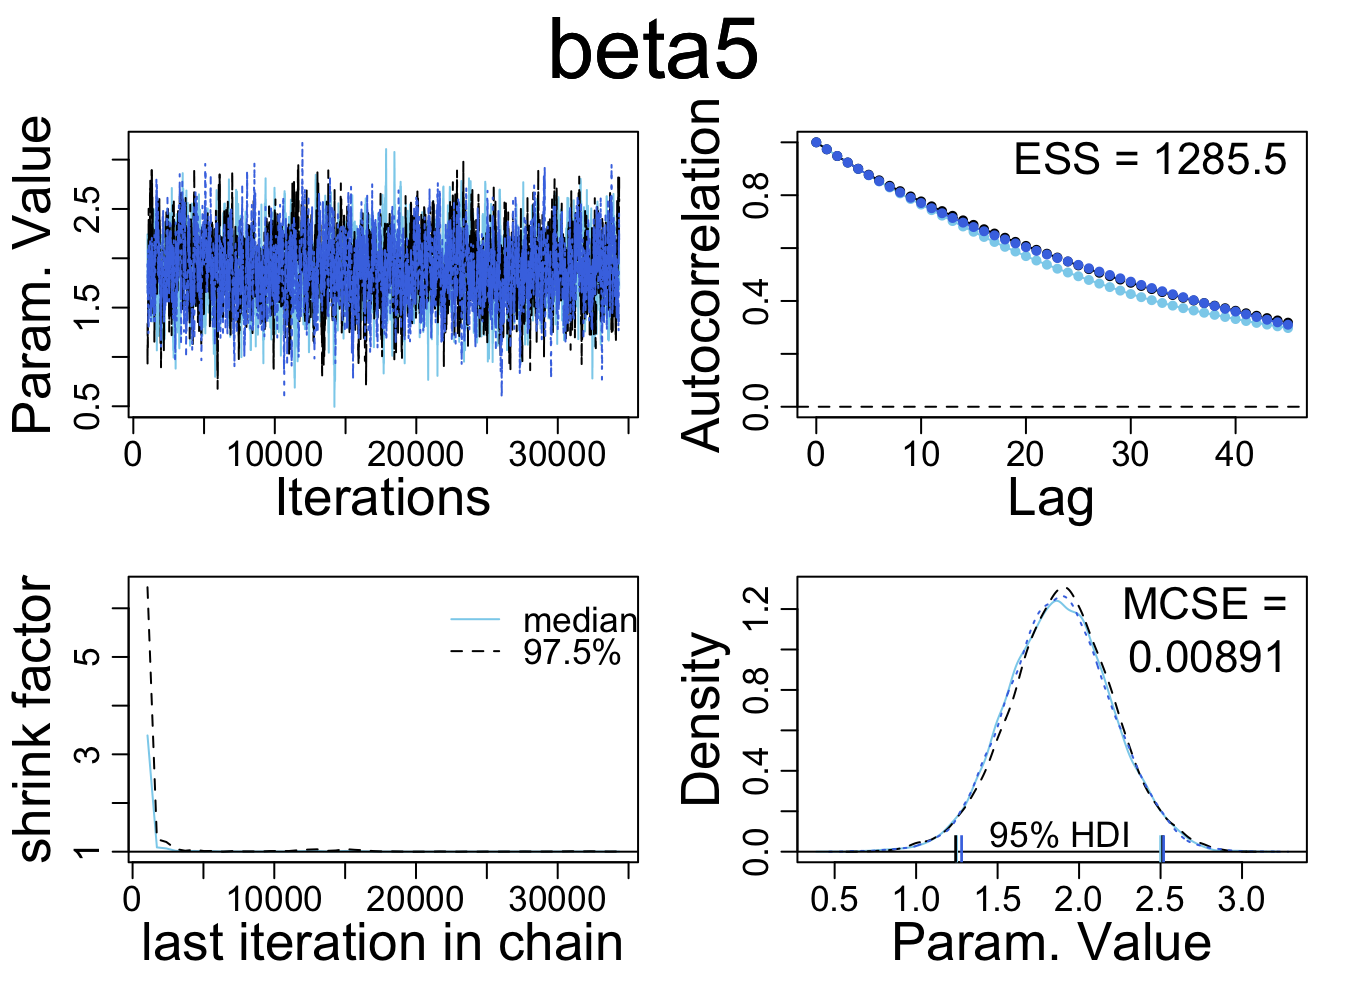
\includegraphics[scale = 0.25]{beta5.png}
\caption{Management Rank}
\label{fig:subim2}
\end{subfigure}
\label{fig:beta1}
\end{figure}

\begin{figure}[h]
 
\begin{subfigure}{0.5\textwidth}
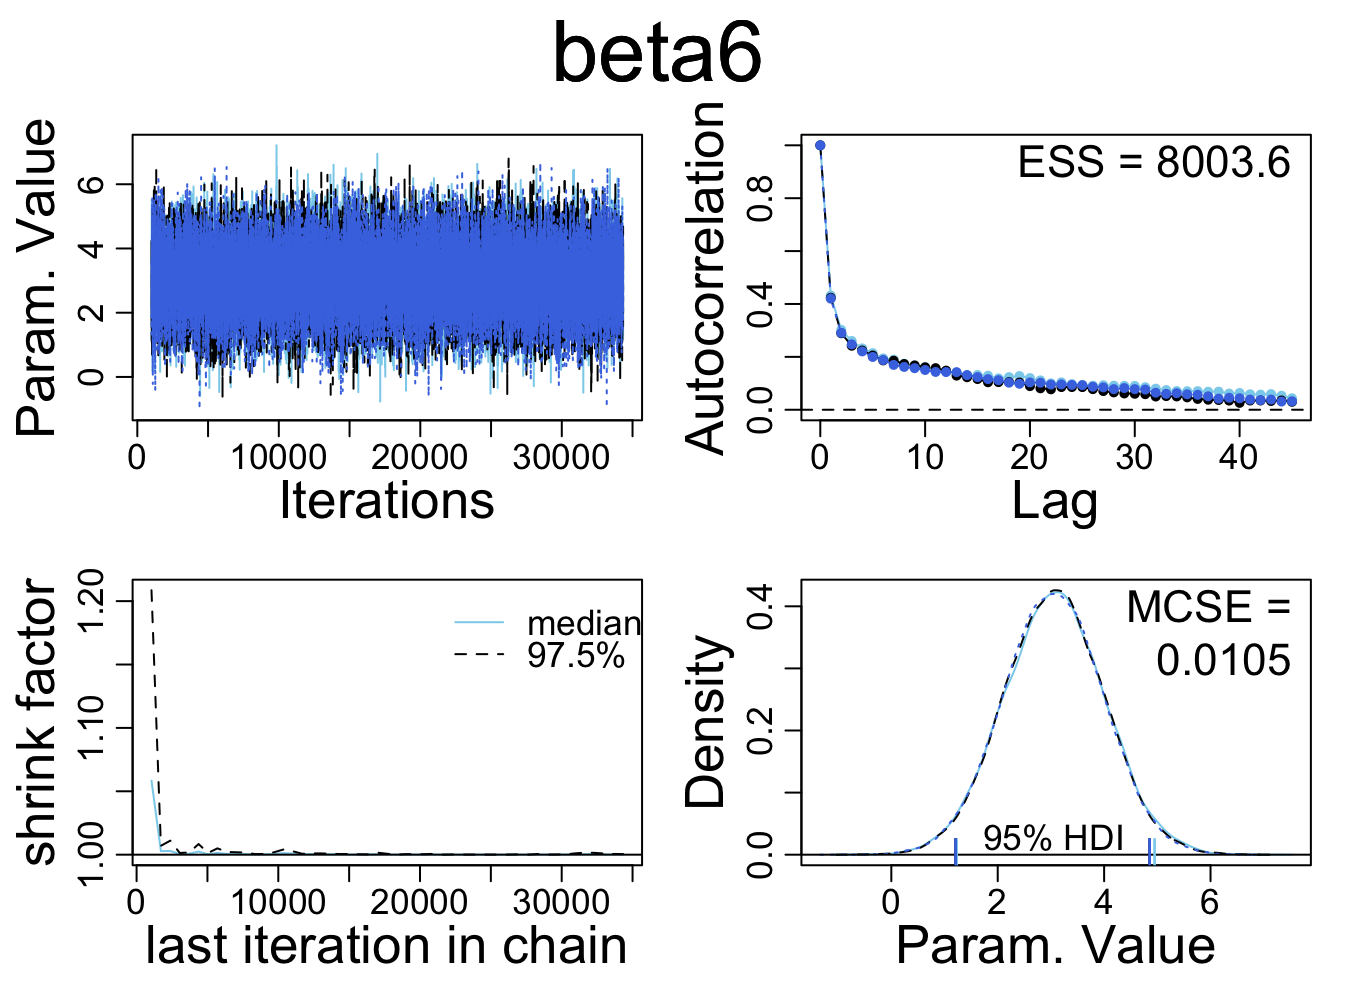
\includegraphics[scale = 0.25]{beta6.png} 
\caption{Luxury Tax}
\label{fig:beta0}
\end{subfigure}
\begin{subfigure}{0.5\textwidth}
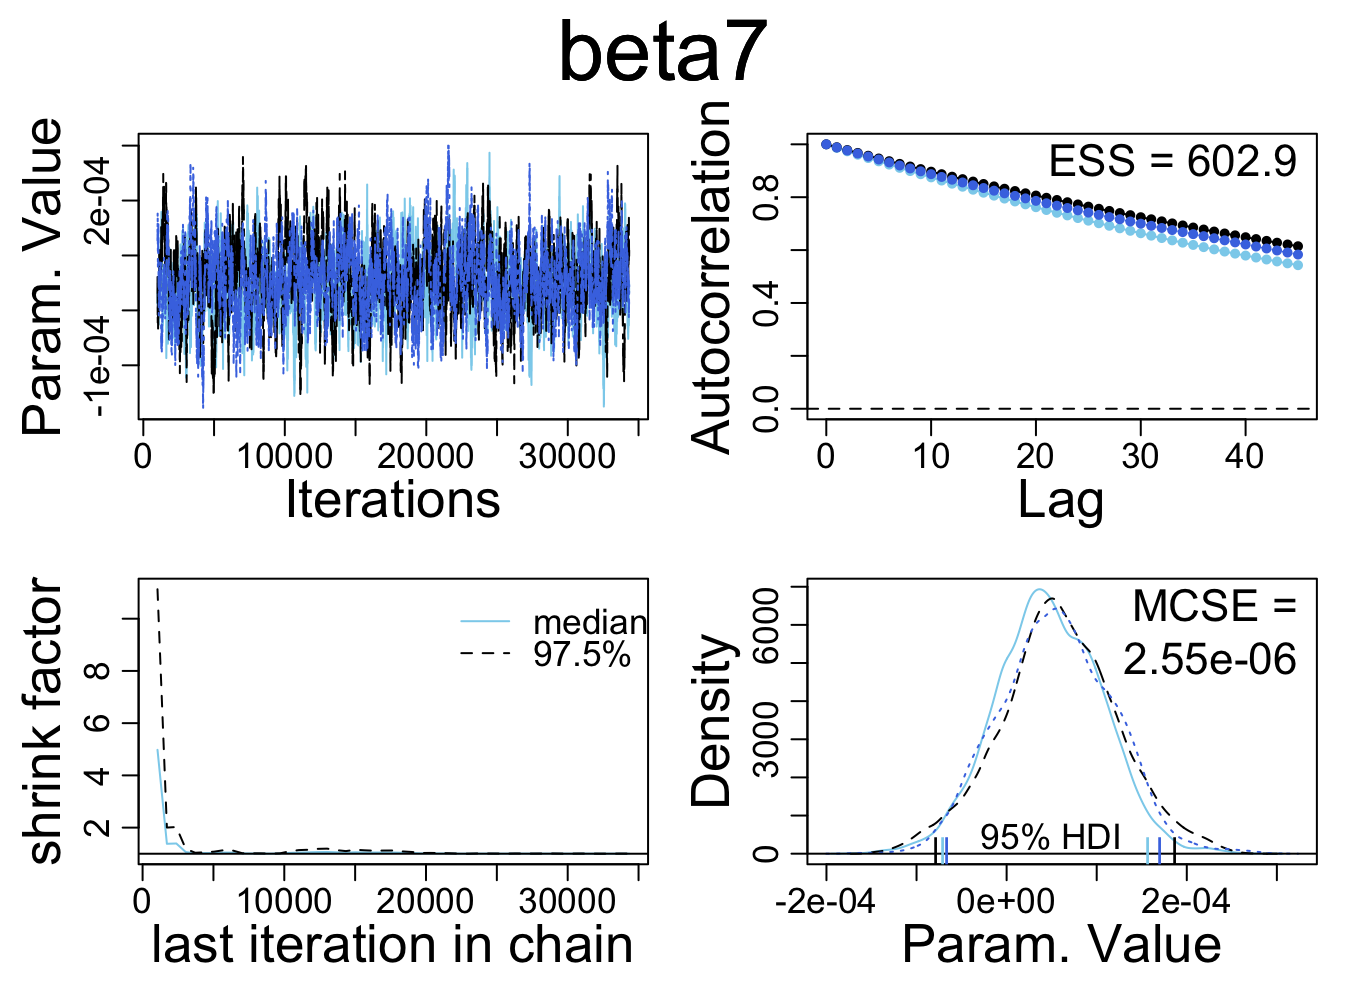
\includegraphics[scale = 0.25]{beta7.png}
\caption{Miles Traveled}
\label{fig:subim2}
\end{subfigure}
\label{fig:beta1}
\end{figure}

\begin{figure}[h]
 
\begin{subfigure}{0.5\textwidth}
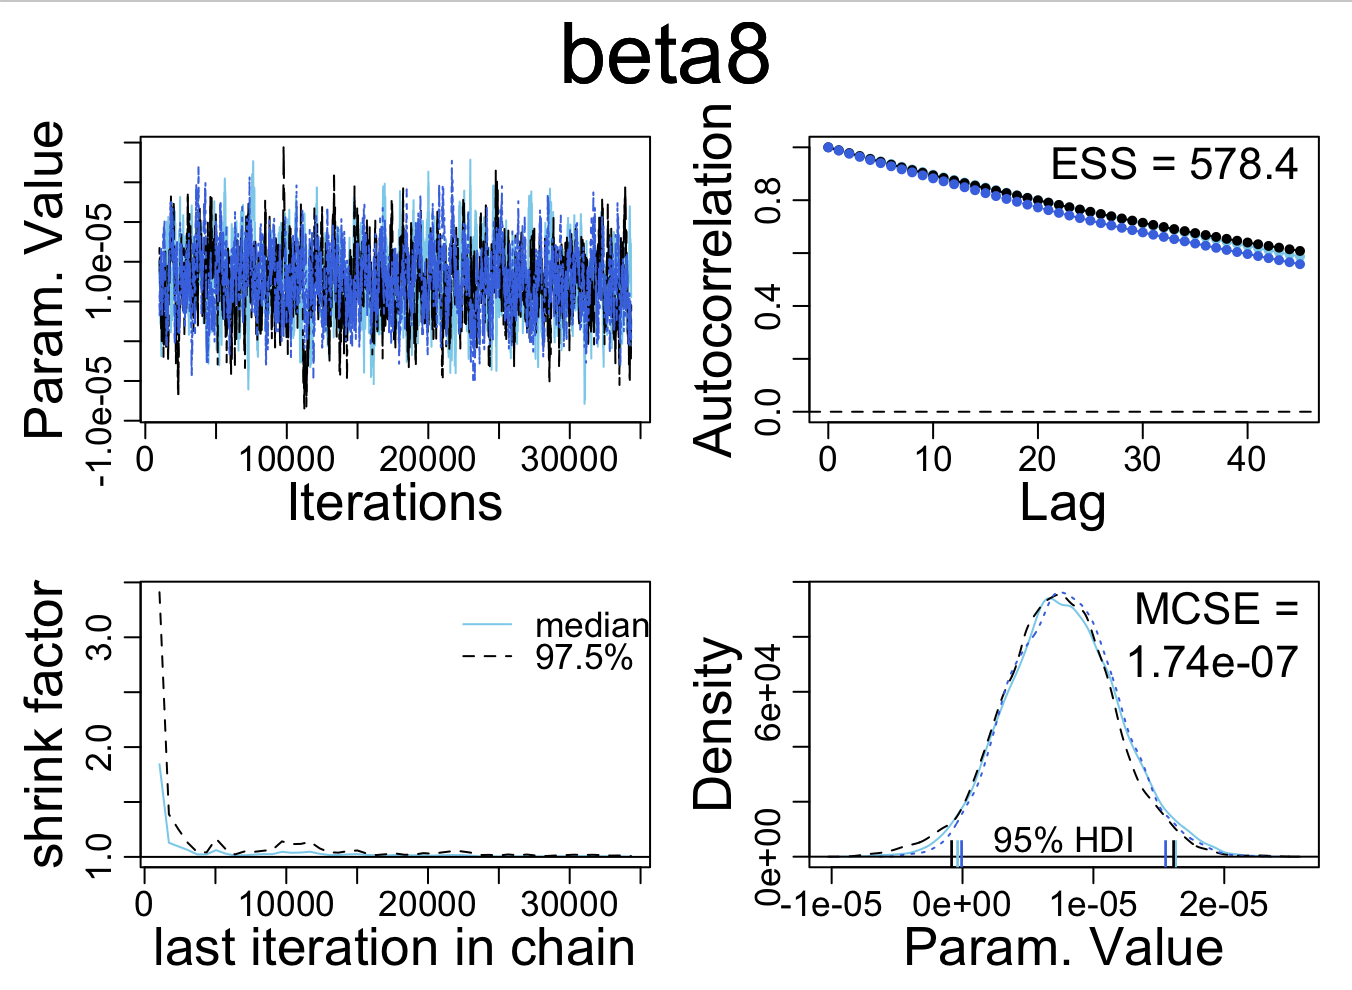
\includegraphics[scale = 0.25]{beta8.png} 
\caption{Fan Attendance}
\label{fig:beta0}
\end{subfigure}
\begin{subfigure}{0.5\textwidth}
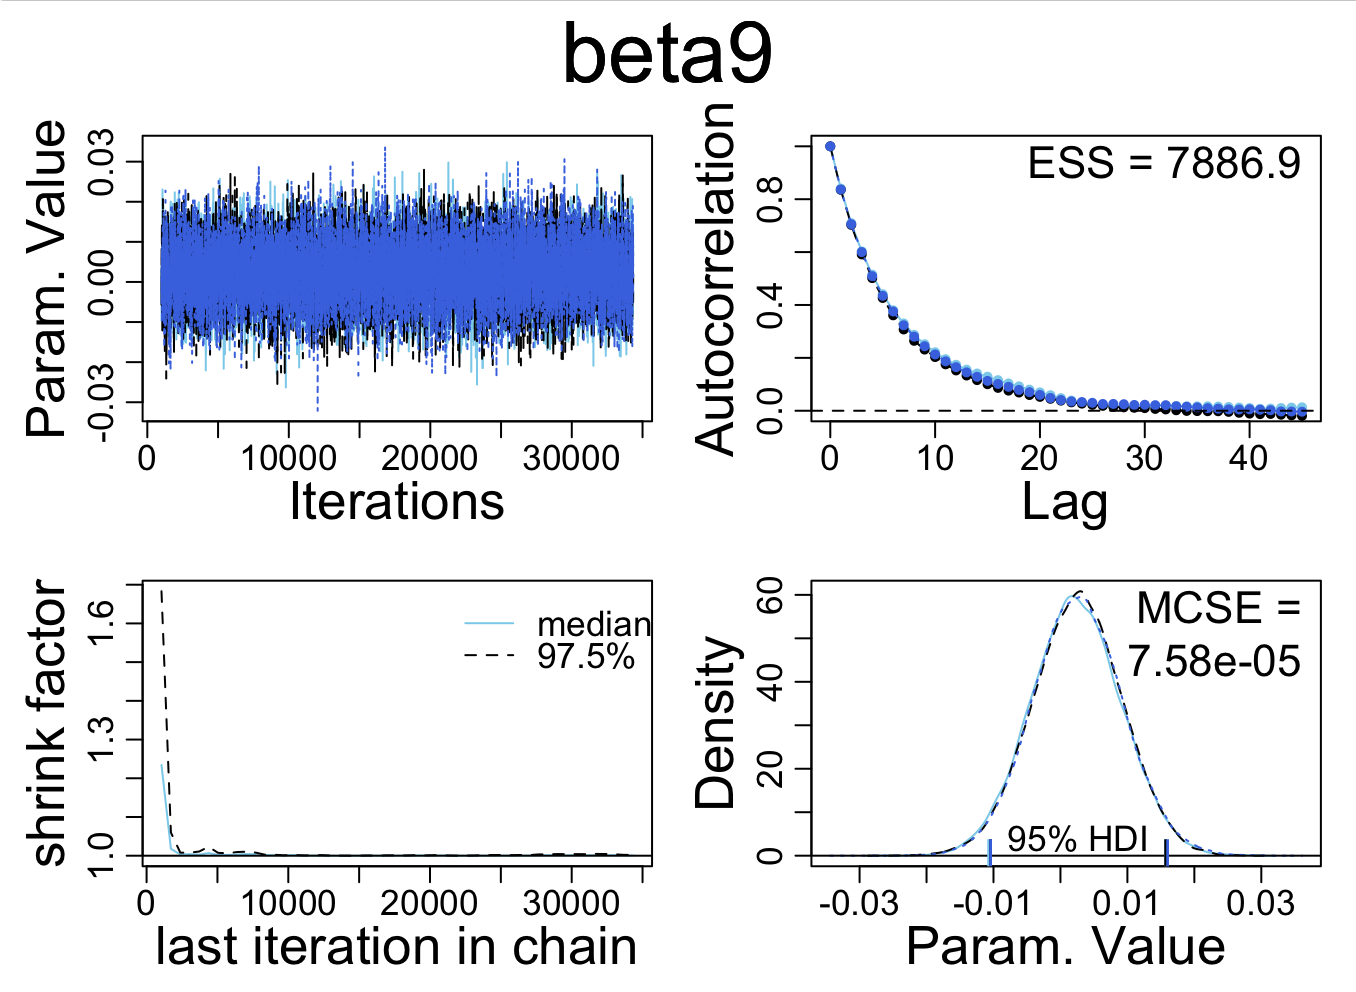
\includegraphics[scale = 0.25]{beta9.png}
\caption{Ticket Price}
\label{fig:subim2}
\end{subfigure}
\label{fig:beta1}
\end{figure}

\begin{figure}[h]
 
\begin{subfigure}{0.5\textwidth}
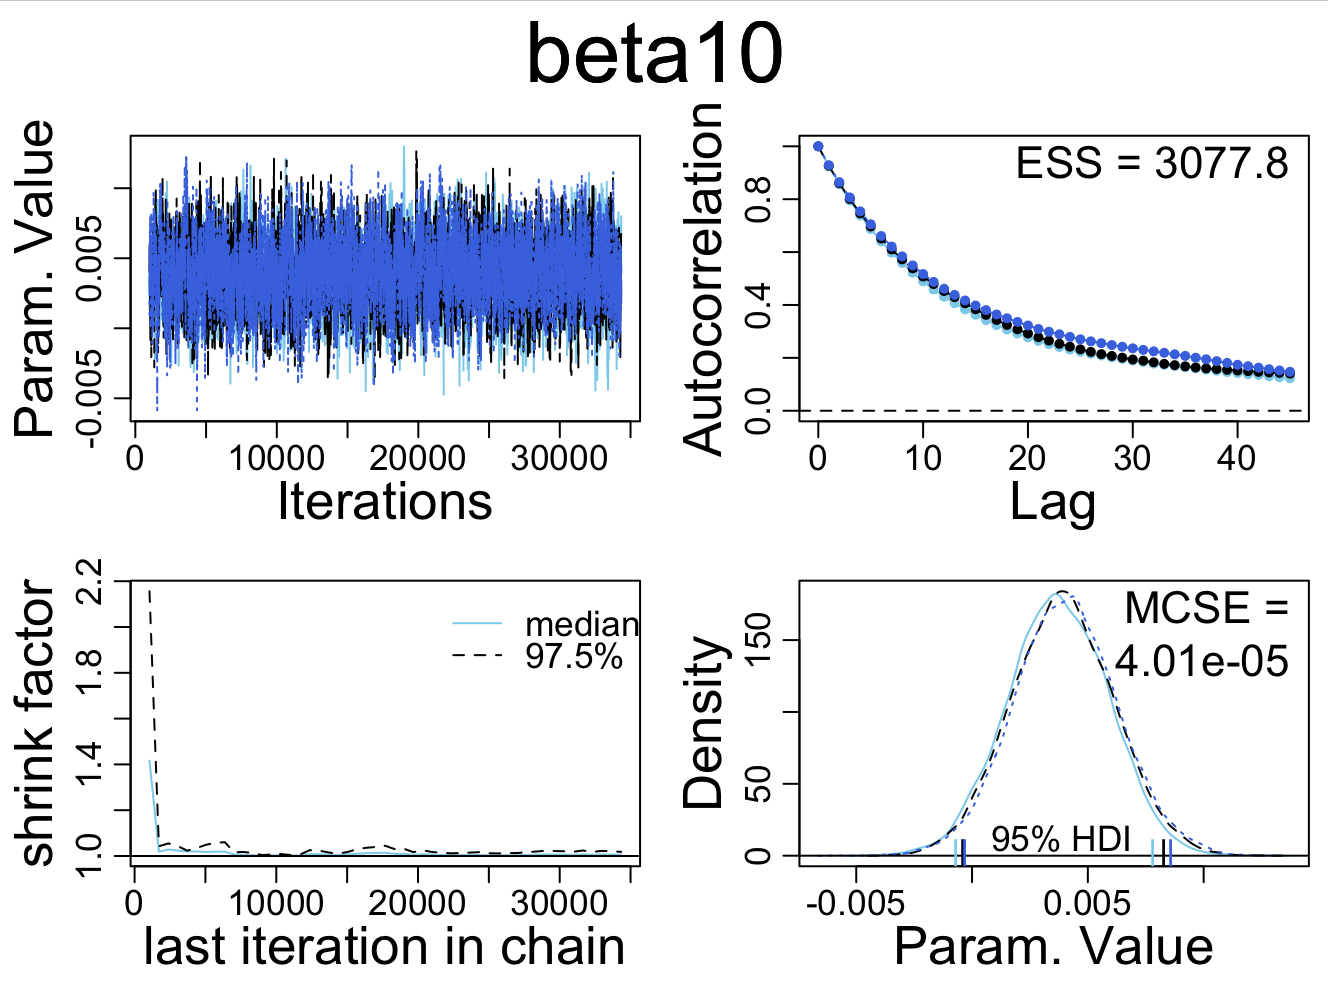
\includegraphics[scale = 0.25]{beta10.png} 
\caption{Crime Index}
\label{fig:beta0}
\end{subfigure}
\begin{subfigure}{0.5\textwidth}
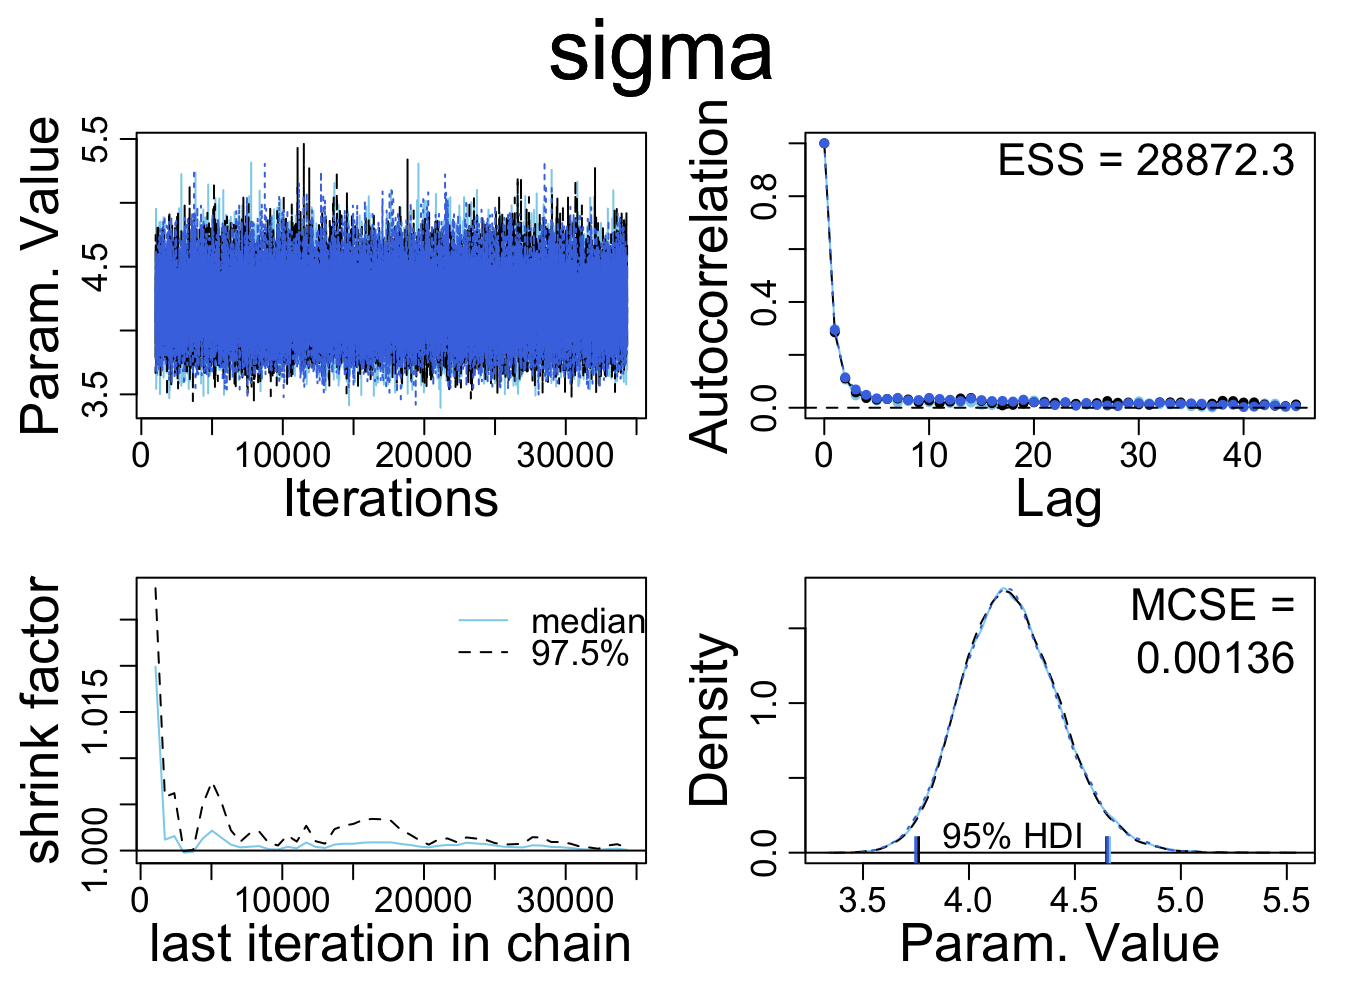
\includegraphics[scale = 0.25]{sigma.png}
\caption{Sigma}
\label{fig:subim2}
\end{subfigure}
\label{fig:beta1}
\end{figure}

\begin{figure}[h]
\caption{Auto Correlations between vairables }
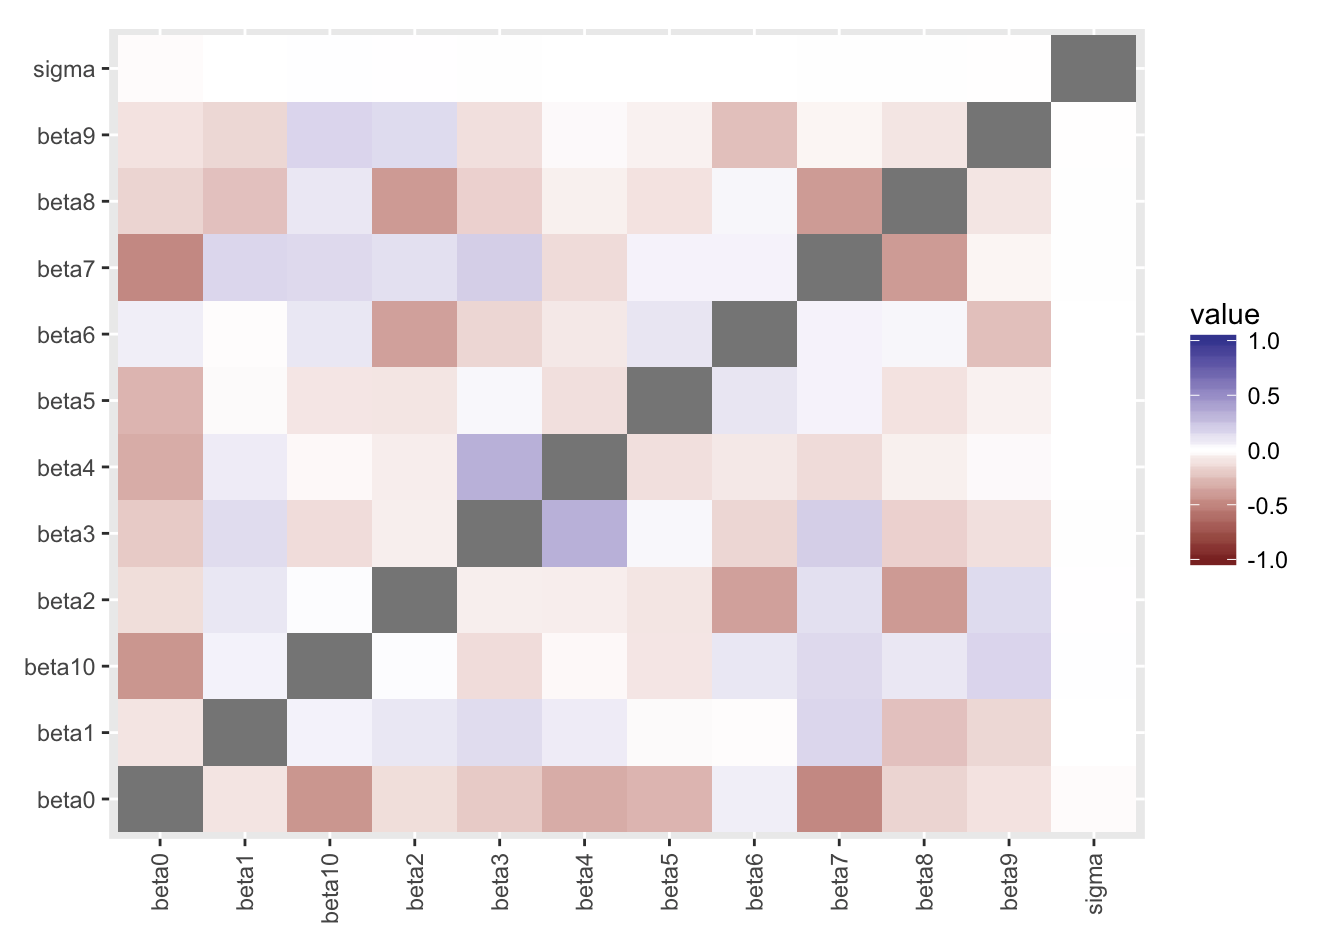
\includegraphics[scale=0.5]{Correlation.png}
\centering
\end{figure}

\end{document}

